\documentclass[11pt, a4paper]{article}
\usepackage[utf8]{inputenc}
\usepackage[left=2.35cm, right=3.35cm, top=3.35cm, bottom=3.0cm]{geometry}
\usepackage{amsmath, amssymb, amsthm}
\usepackage[english]{babel}
\usepackage{graphicx}
\usepackage[font={small,it}]{caption}
\graphicspath{ {figures/} }
\usepackage{url}
\usepackage{appendix}
\usepackage{float}
\usepackage{multirow}
\usepackage[bottom]{footmisc}
\usepackage{titling}
\usepackage{subcaption}
\usepackage{wrapfig}
\usepackage[numbered,autolinebreaks,useliterate]{mcode}
\begin{document}

\begin{titlepage}
  \begin{center}
    
    
\includegraphics[scale=1.5]{figures/kuleuven_logo.pdf}~\\[4.5cm]
    \textsc{\Large Master of bioinformatics}\\[0.5cm]

    % Title
    \rule{\linewidth}{0.3mm}\\[0.4cm]
    {\huge \bfseries Support Vector Machines} \\[0.4cm]
    {\large Assignment 3: Unsupervised Learning} \\[0.4cm]
    \rule{\linewidth}{0.3mm}\\[0.4cm]
    {\large Spring 2016} \\[1.0cm]
    
    % Author and supervisor
    \begin{minipage}{0.4\textwidth}
      \begin{flushleft} \large
        \emph{Author:}\\
	Cedric \textsc{Lood}
      \end{flushleft}
    \end{minipage}
%     %\hfill
    \begin{minipage}{0.4\textwidth}
      \begin{flushright} \large
        \emph{Supervisors:} \\
        Dr. Carlos \textsc{Alaiz}\\
        Dr. Emanuele \textsc{Frandi}\\
        Prof. Johan \textsc{Suykens}\\
        \hfill \newline 
      \end{flushright}
    \end{minipage}
    
    \vfill

    
\includegraphics[scale=0.15]{figures/KUL.jpg}~\\[0.5cm]

    % Bottom of the page
    {\large \today}
    
  \end{center}
\end{titlepage}

\tableofcontents
\newpage

\section*{Context}

The analysis presented in this report was produced for the class of
``Support Vector Machines: methods and applications'' at KU Leuven
(Spring 2016). The goal is to display understanding of the principles
behind support vector machines and of how to work out good solutions
using these techniques. This third report focuses on unsupervised
learning (kernel PCA) using Least-Squares SVM (LS-SVM). The
implementation was done using the MatLab environment (v2015a) and the
libraries for LS-SVM developed at KU Leuven
\footnote{http://www.esat.kuleuven.be/sista/lssvmlab/}.

\section{Kernel Principal Component Analysis}

In this section, we explore the synthetic dataset illustrated on
figure \ref{fig:kpca_dataset} to explore the relationship between the
choices of kernel, hyper-parameters and the number of components. 

\begin{figure}[H]
  \centering
  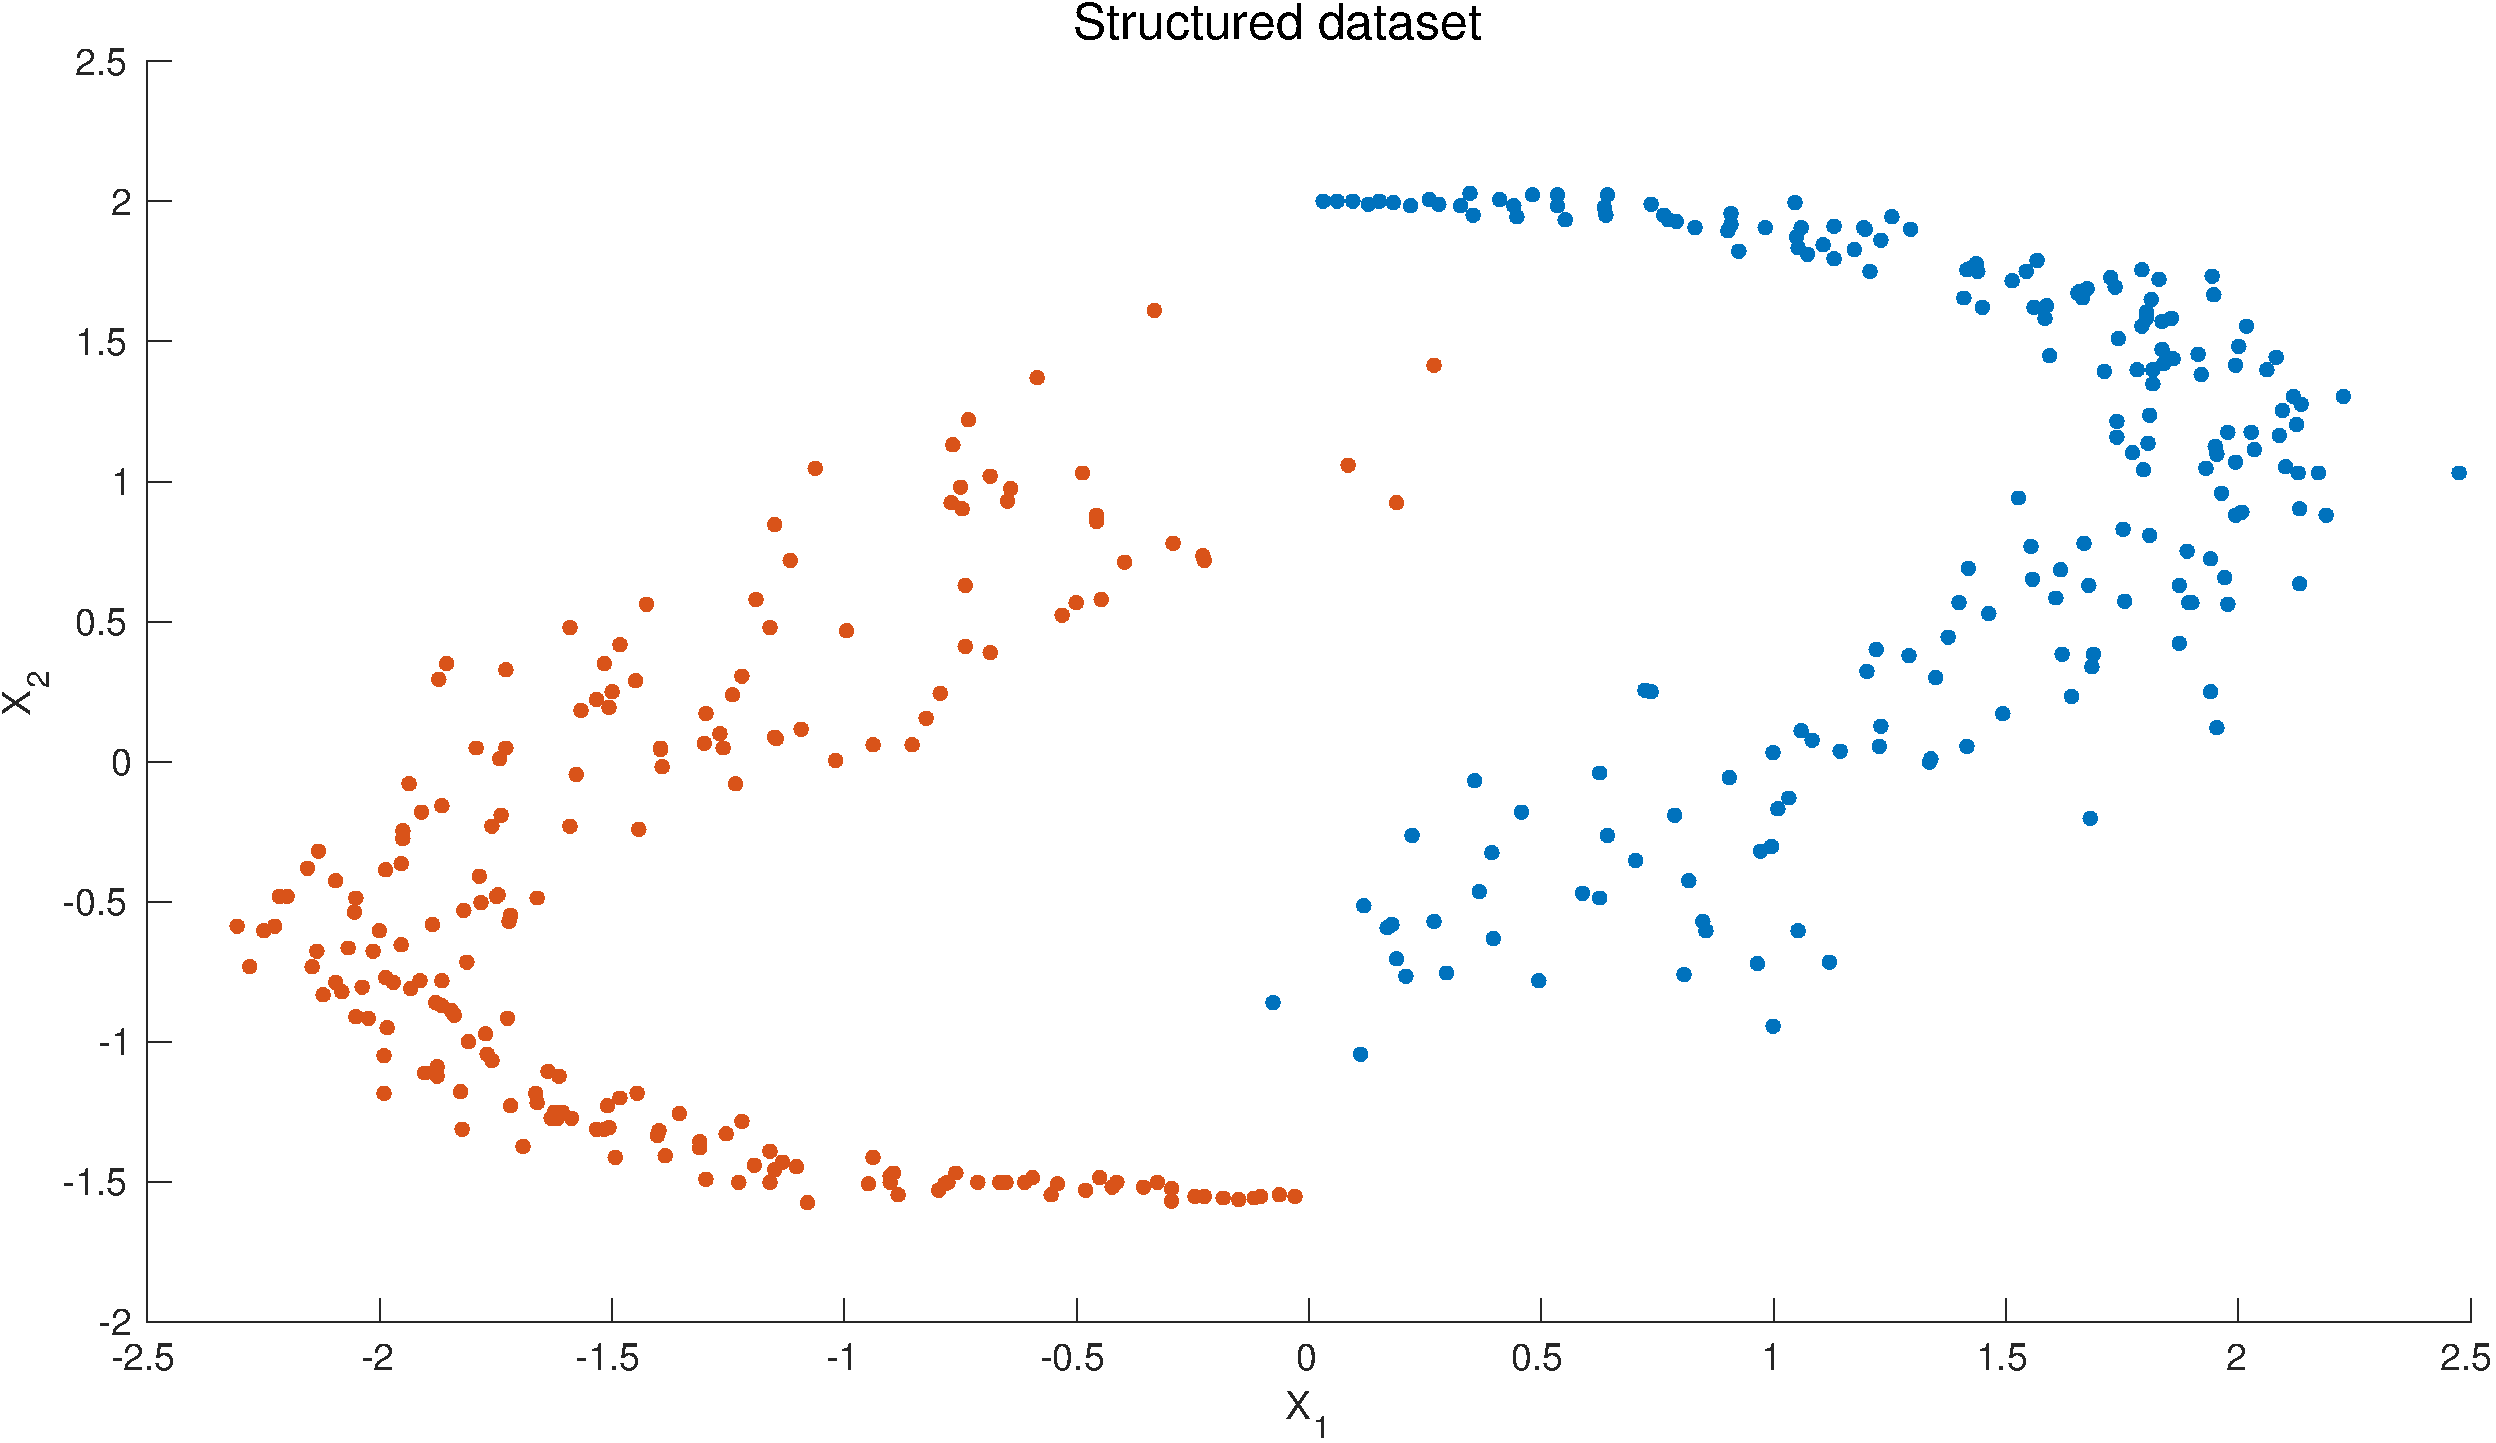
\includegraphics[scale=.40]{kpca_dataset.pdf}
  \caption{Synthetic dataset Yin-Yang}
  \label{fig:kpca_dataset}
\end{figure}

Figure \ref{fig:kpca_ncomp} allows us to visualize what happens when
you increase the number of component in a given setting (here
$\sigma^2=0.4$). We can see that the denoising works really well once
the number of components has increased to 4 and above. Figure
\ref{fig:kpca_sigma} illustrates the impact of $\sigma^2$ on the
denoising for a number of components fixed to 6.

Given the structure of the dataset, linear PCA gives very poor results
in terms of denoising (see figure \ref{fig:kpca_linear}). The maximum
amount of principal component that can be obtained using linear PCA
corresponds to the dimensionality of the original input space. For the
kernel PCA, since we are working in the feature space, the
dimensionality can be higher, and corresponds to the dimensionality of
the kernel matrix.


\begin{figure}[H]
  \centering
  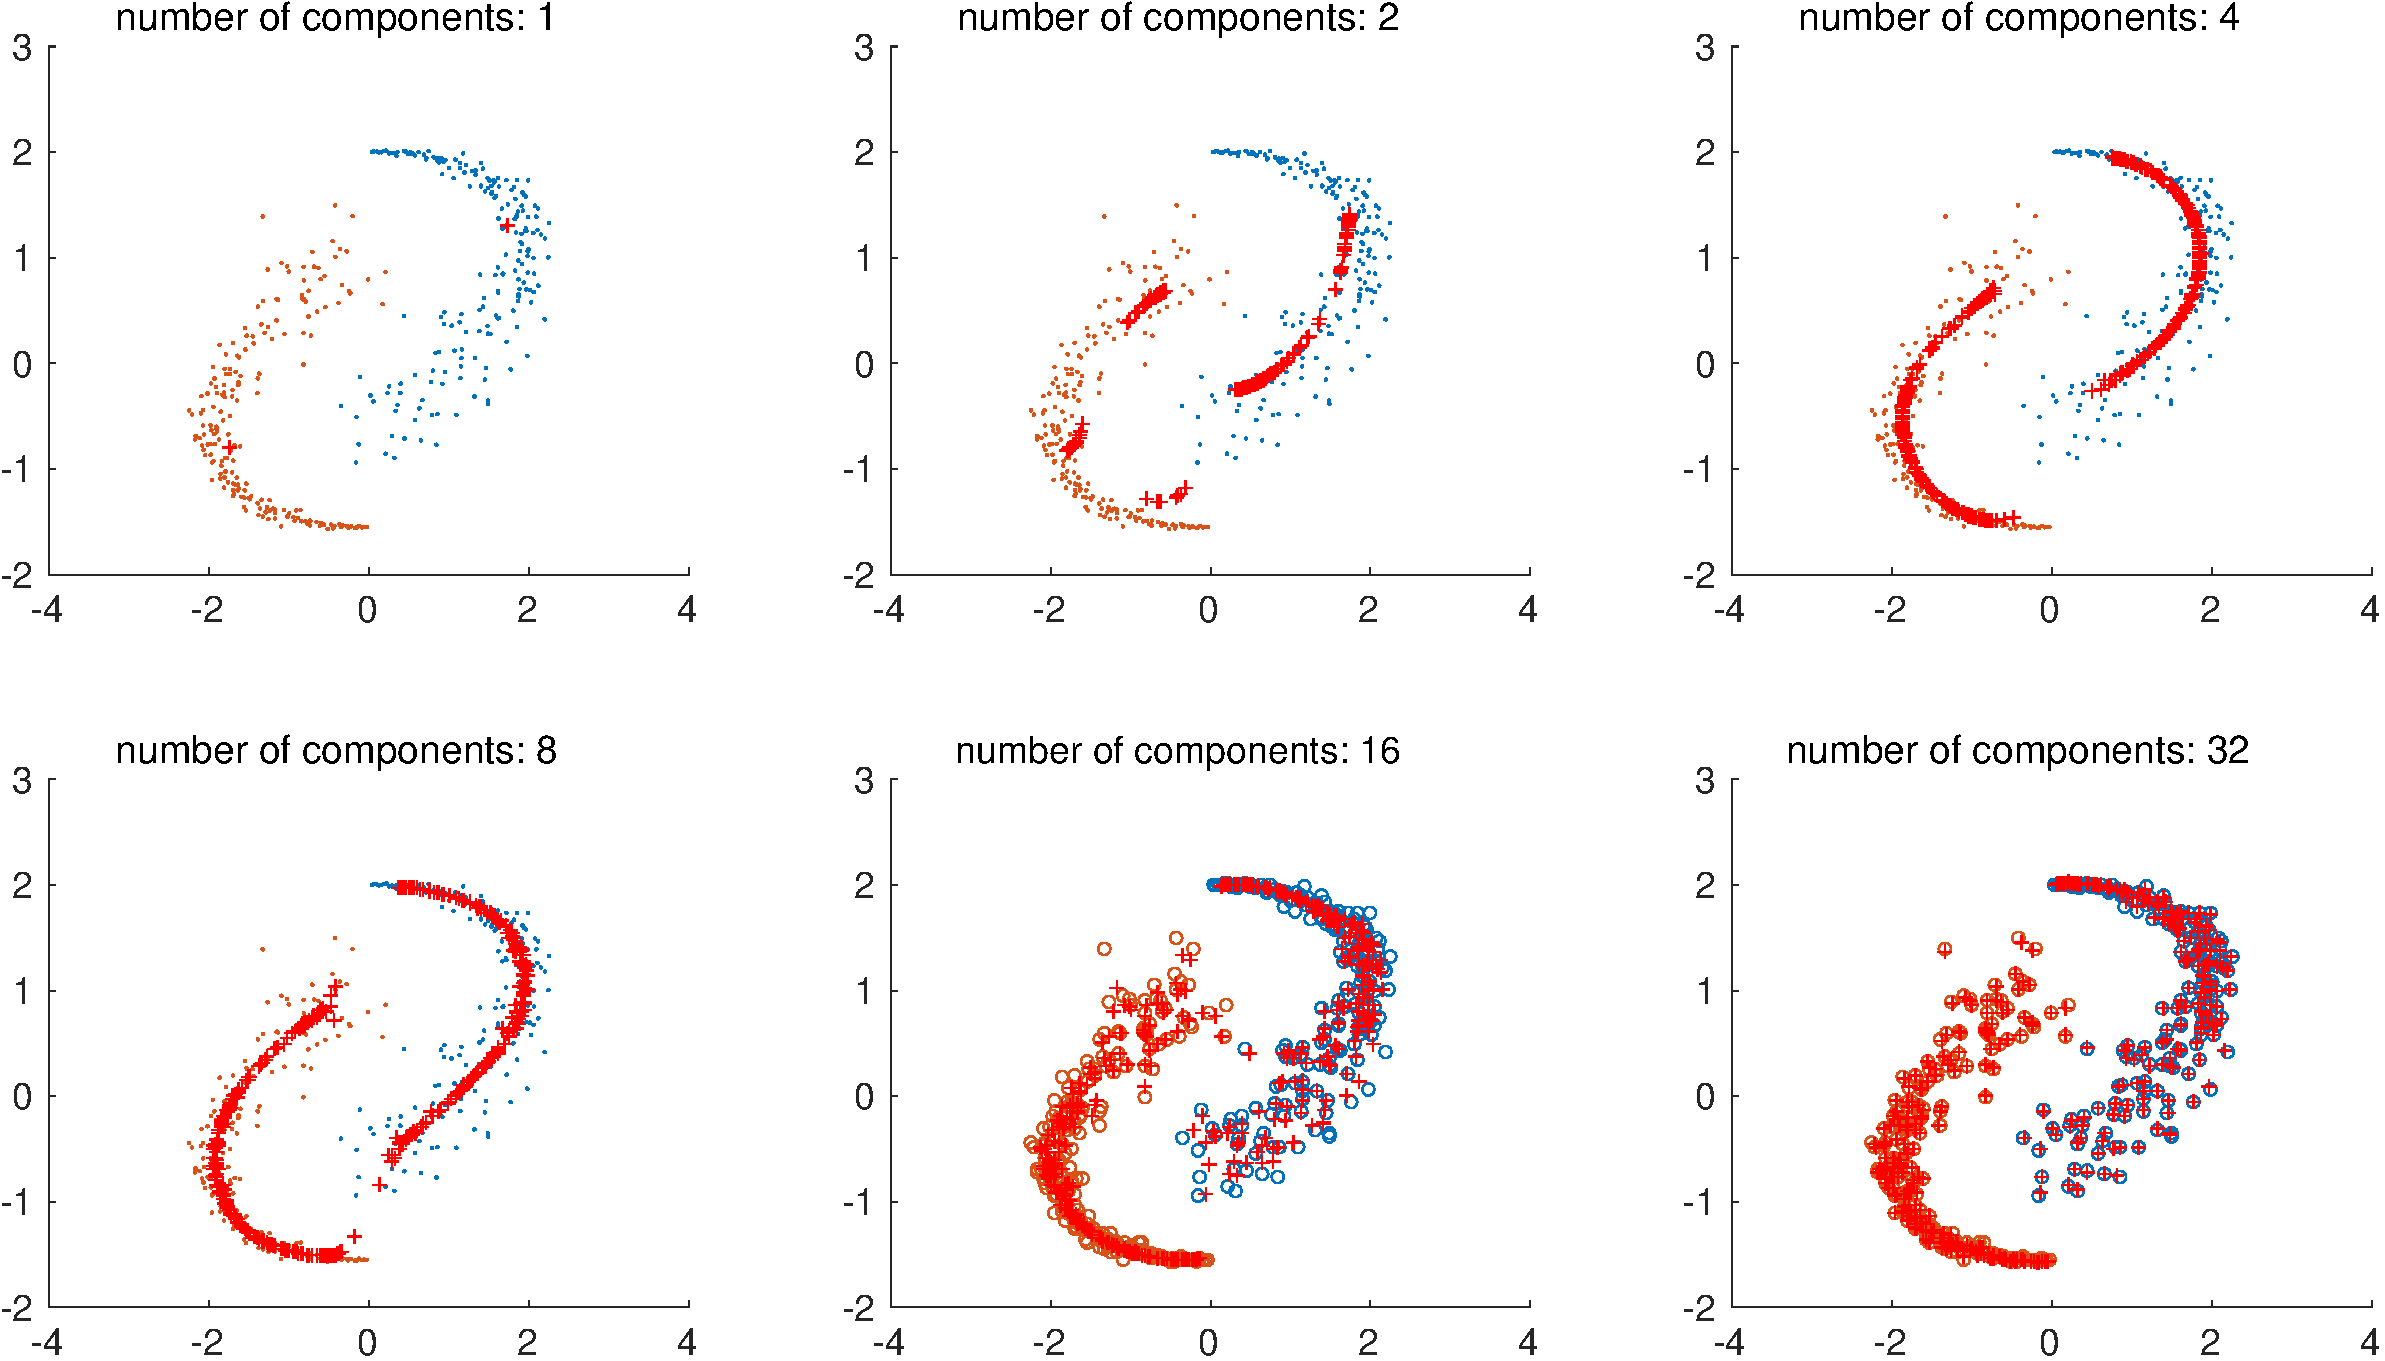
\includegraphics[scale=.40]{kpca_ncomp.pdf}
  \caption{Denoising for various values of components}
  \label{fig:kpca_ncomp}
\end{figure}

\begin{figure}[H]
  \centering
  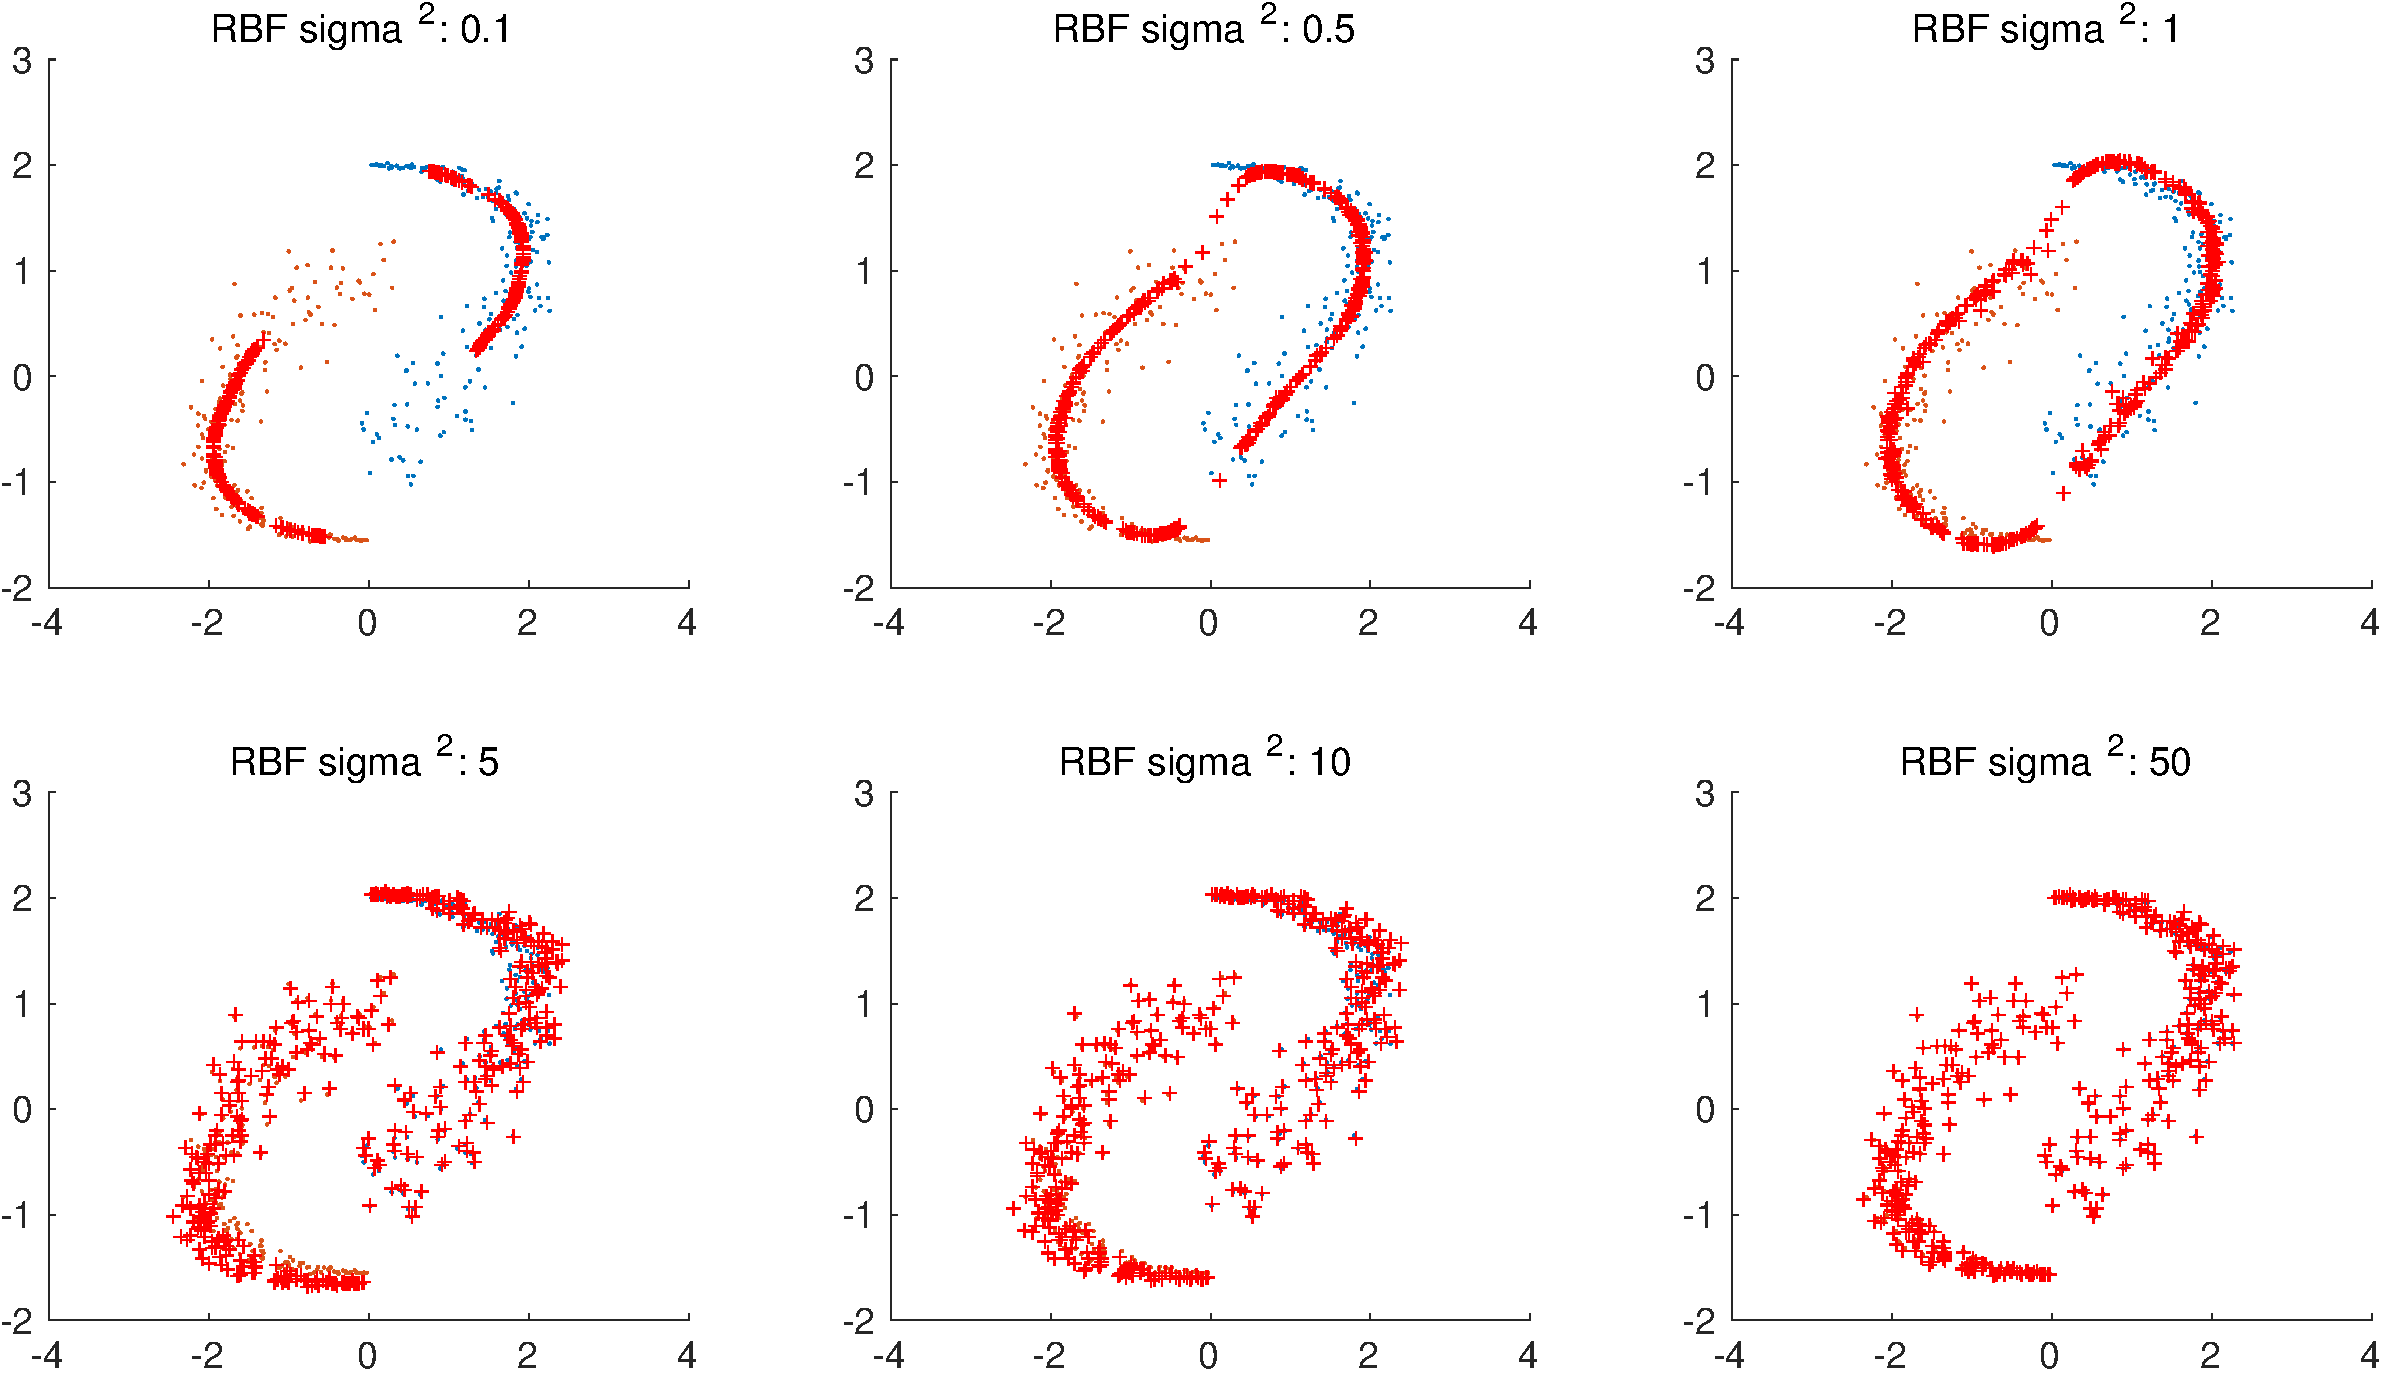
\includegraphics[scale=.40]{kpca_sigma.pdf}
  \caption{Denoising for various values of $\sigma^2$}
  \label{fig:kpca_sigma}
\end{figure}

\begin{figure}[H]
  \centering
  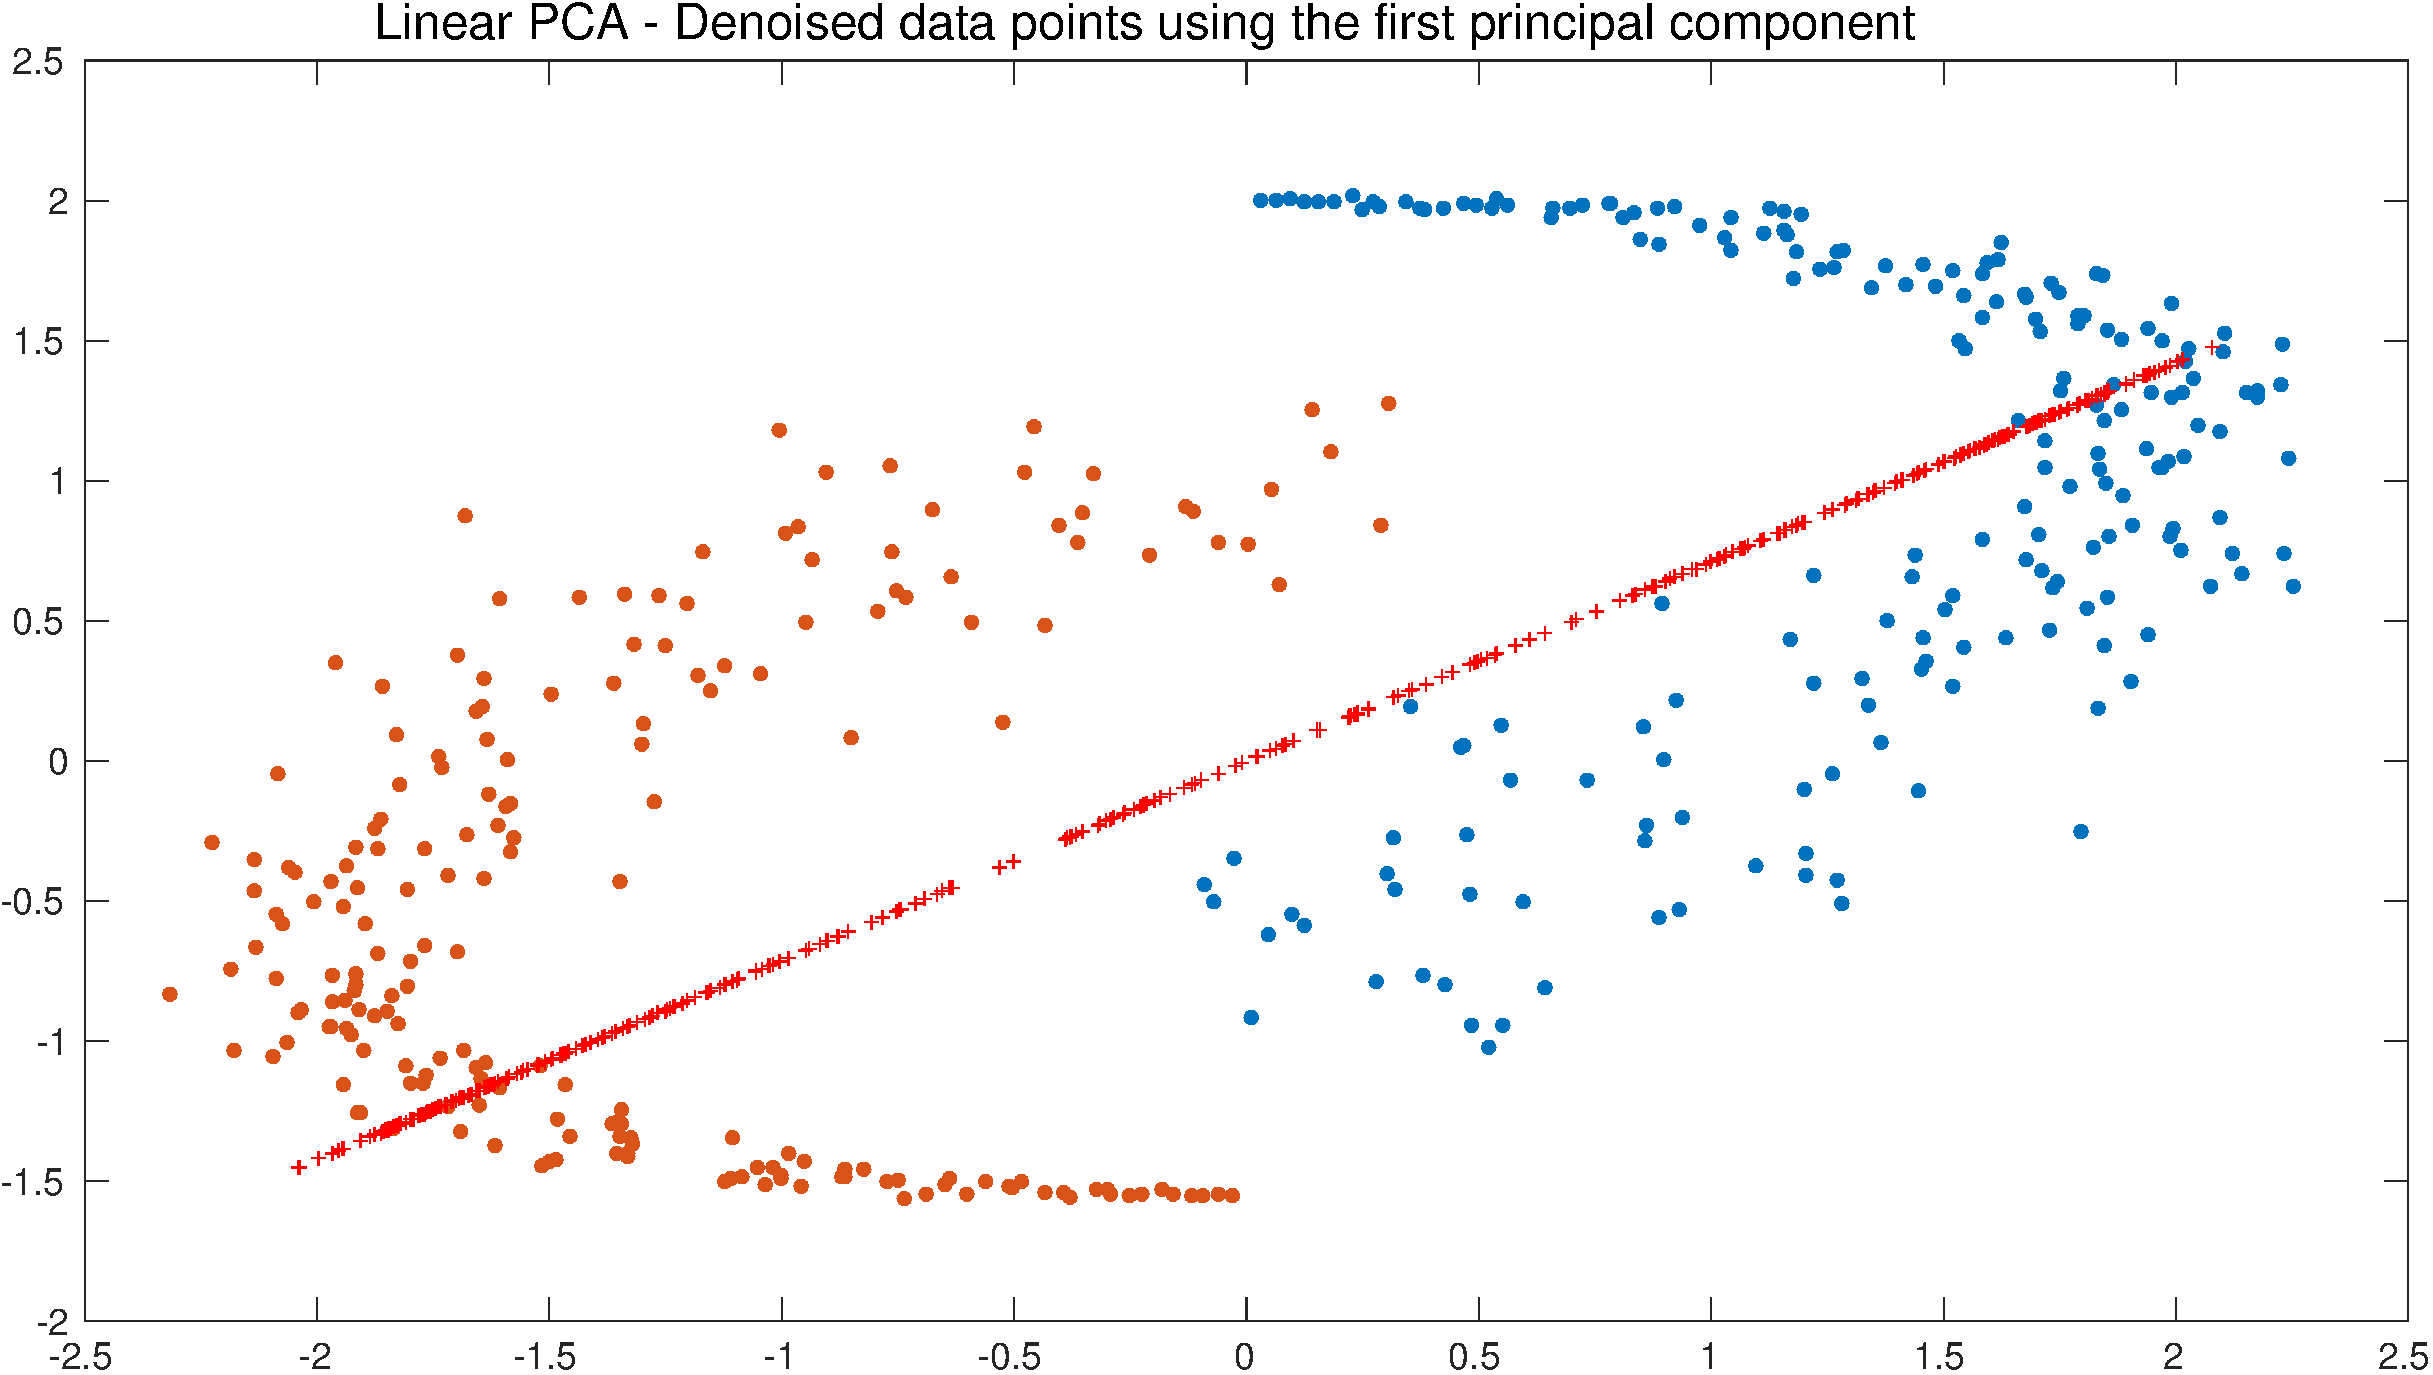
\includegraphics[scale=.30]{kpca_linear.pdf}
  \caption{Denoising in linear PCA setting}
  \label{fig:kpca_linear}
\end{figure}

\section{Handwritten Digit Denoising}

The results of the denoising process are reported on figures
\ref{fig:digitsn_kernelpc} and \ref{fig:digitsn_linearpca}. As can be
observed, the performance of the kernel PCA in terms of denoising are
much better. Basically, the linear PCA decomposition into 256
components, followed by the reconstruction using progressively more
and more components (256 in the last row) returns the original noisy
image. Where as the kernel PCA is able to extract out the gaussian
noise during the reconstruction, returning a very convincing, denoised
image which is similar to the original noiseless one.


\begin{figure}[H]
  \centering
  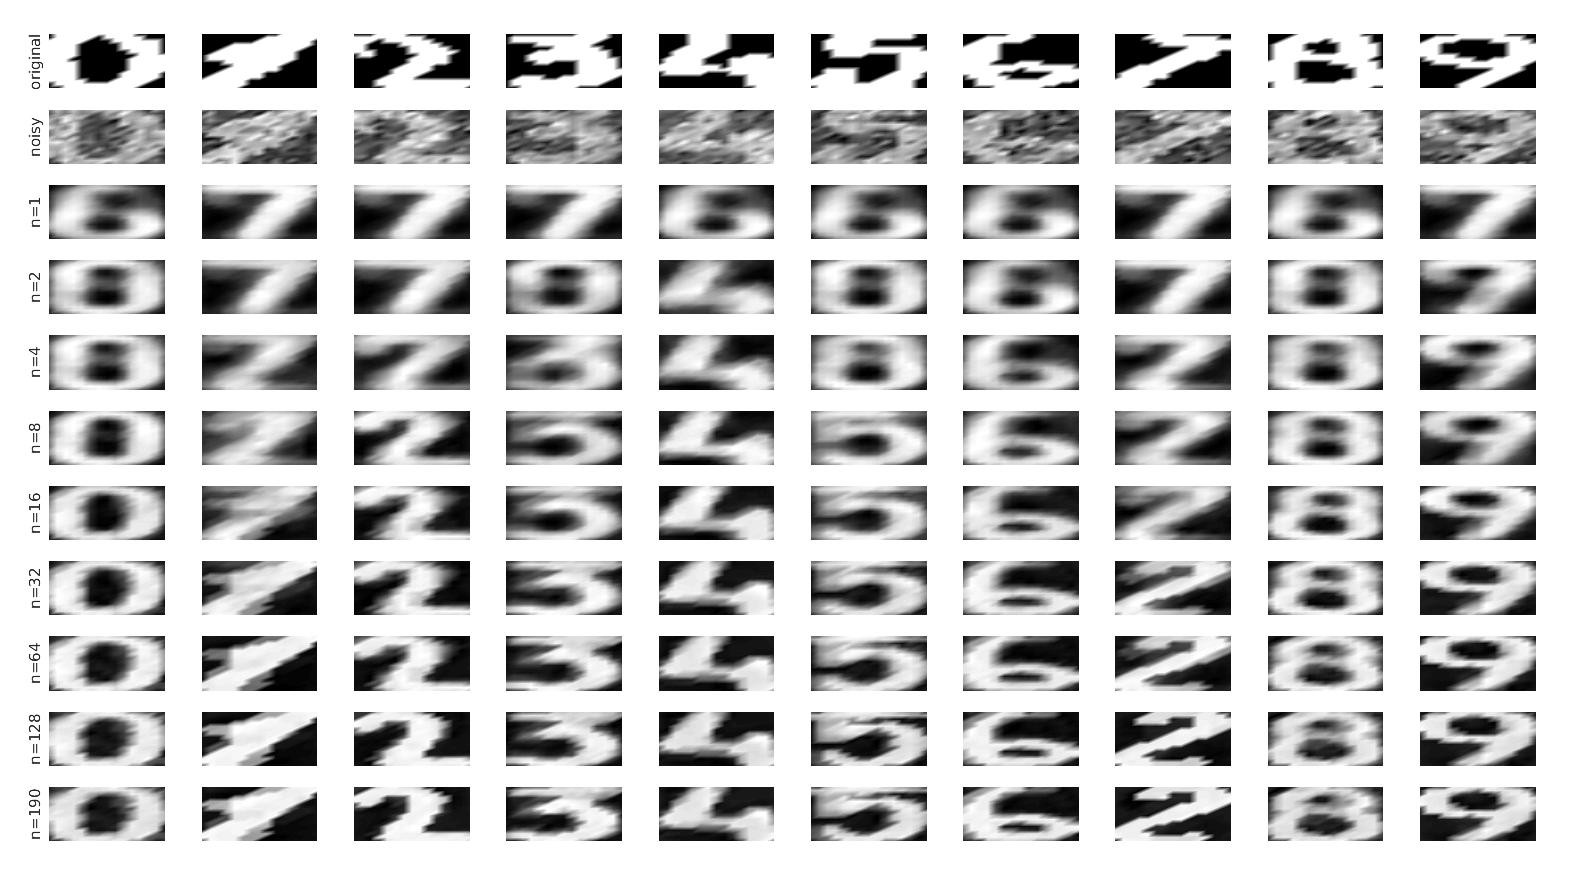
\includegraphics[scale=.30]{digitsn_kernelpca.jpg}
  \caption{Denoising digits using a kernel PCA approach}
  \label{fig:digitsn_kernelpca}
\end{figure}

\begin{figure}[H]
  \centering
  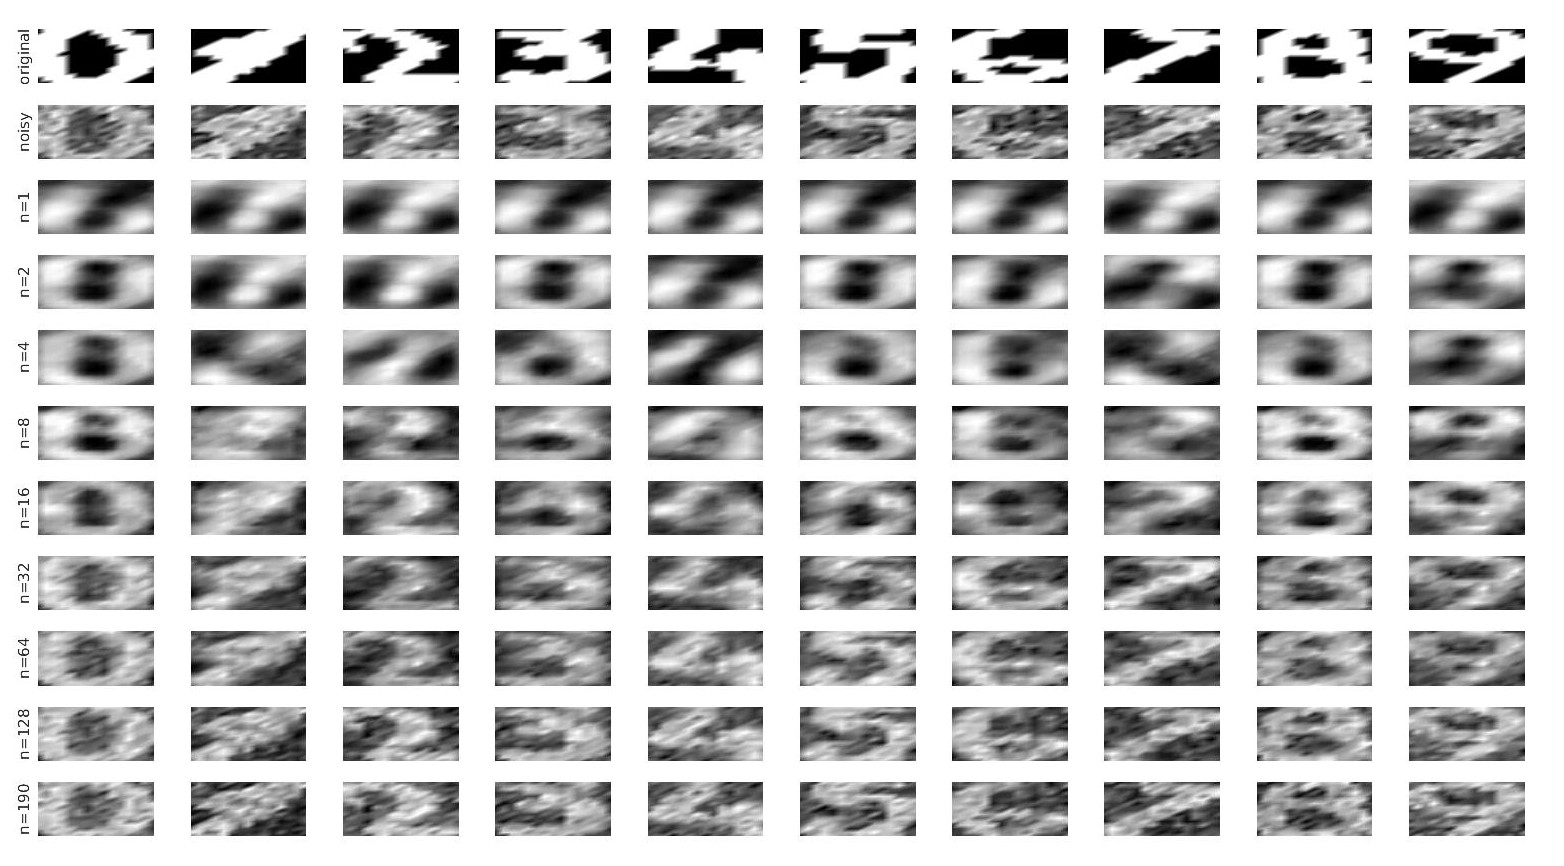
\includegraphics[scale=.30]{digitsn_linearpca.jpg}
  \caption{Denoising digits using a linear PCA approach}
  \label{fig:digitsn_linearpc}
\end{figure}

\section{Spectral Clustering}

\begin{figure}[H]
  \centering
  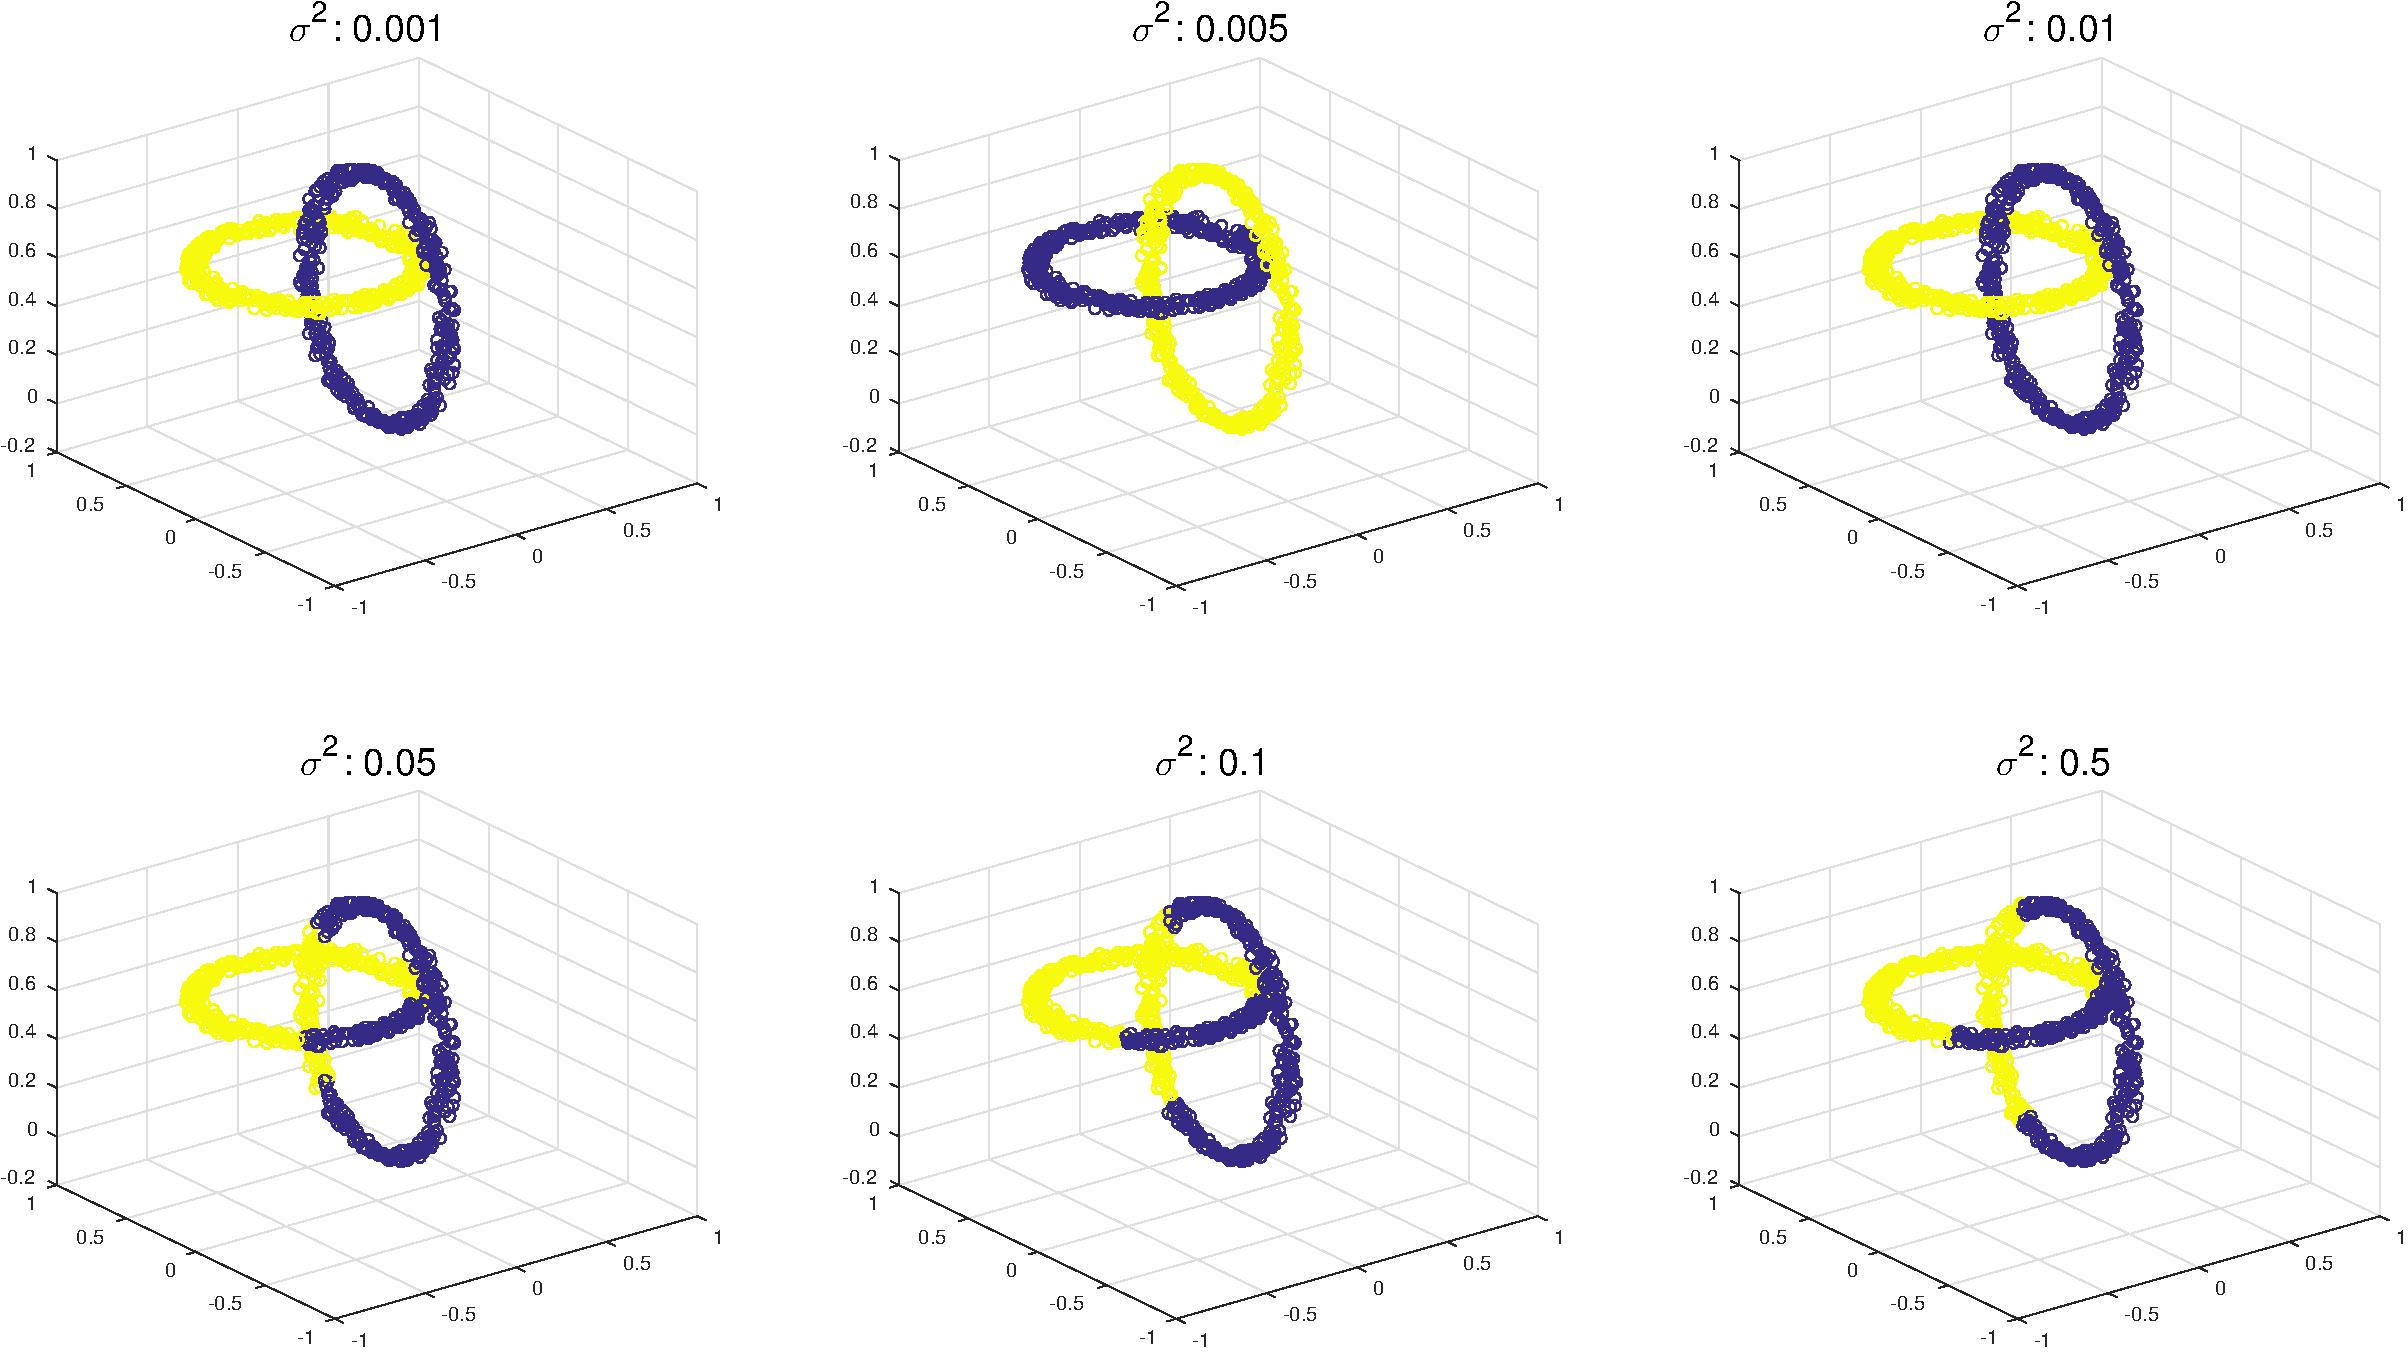
\includegraphics[scale=.40]{sclustering_origcl.pdf}
  \caption{Clustering 1}
  \label{fig:sclustering_origcl}
\end{figure}

\begin{figure}[H]
  \centering
  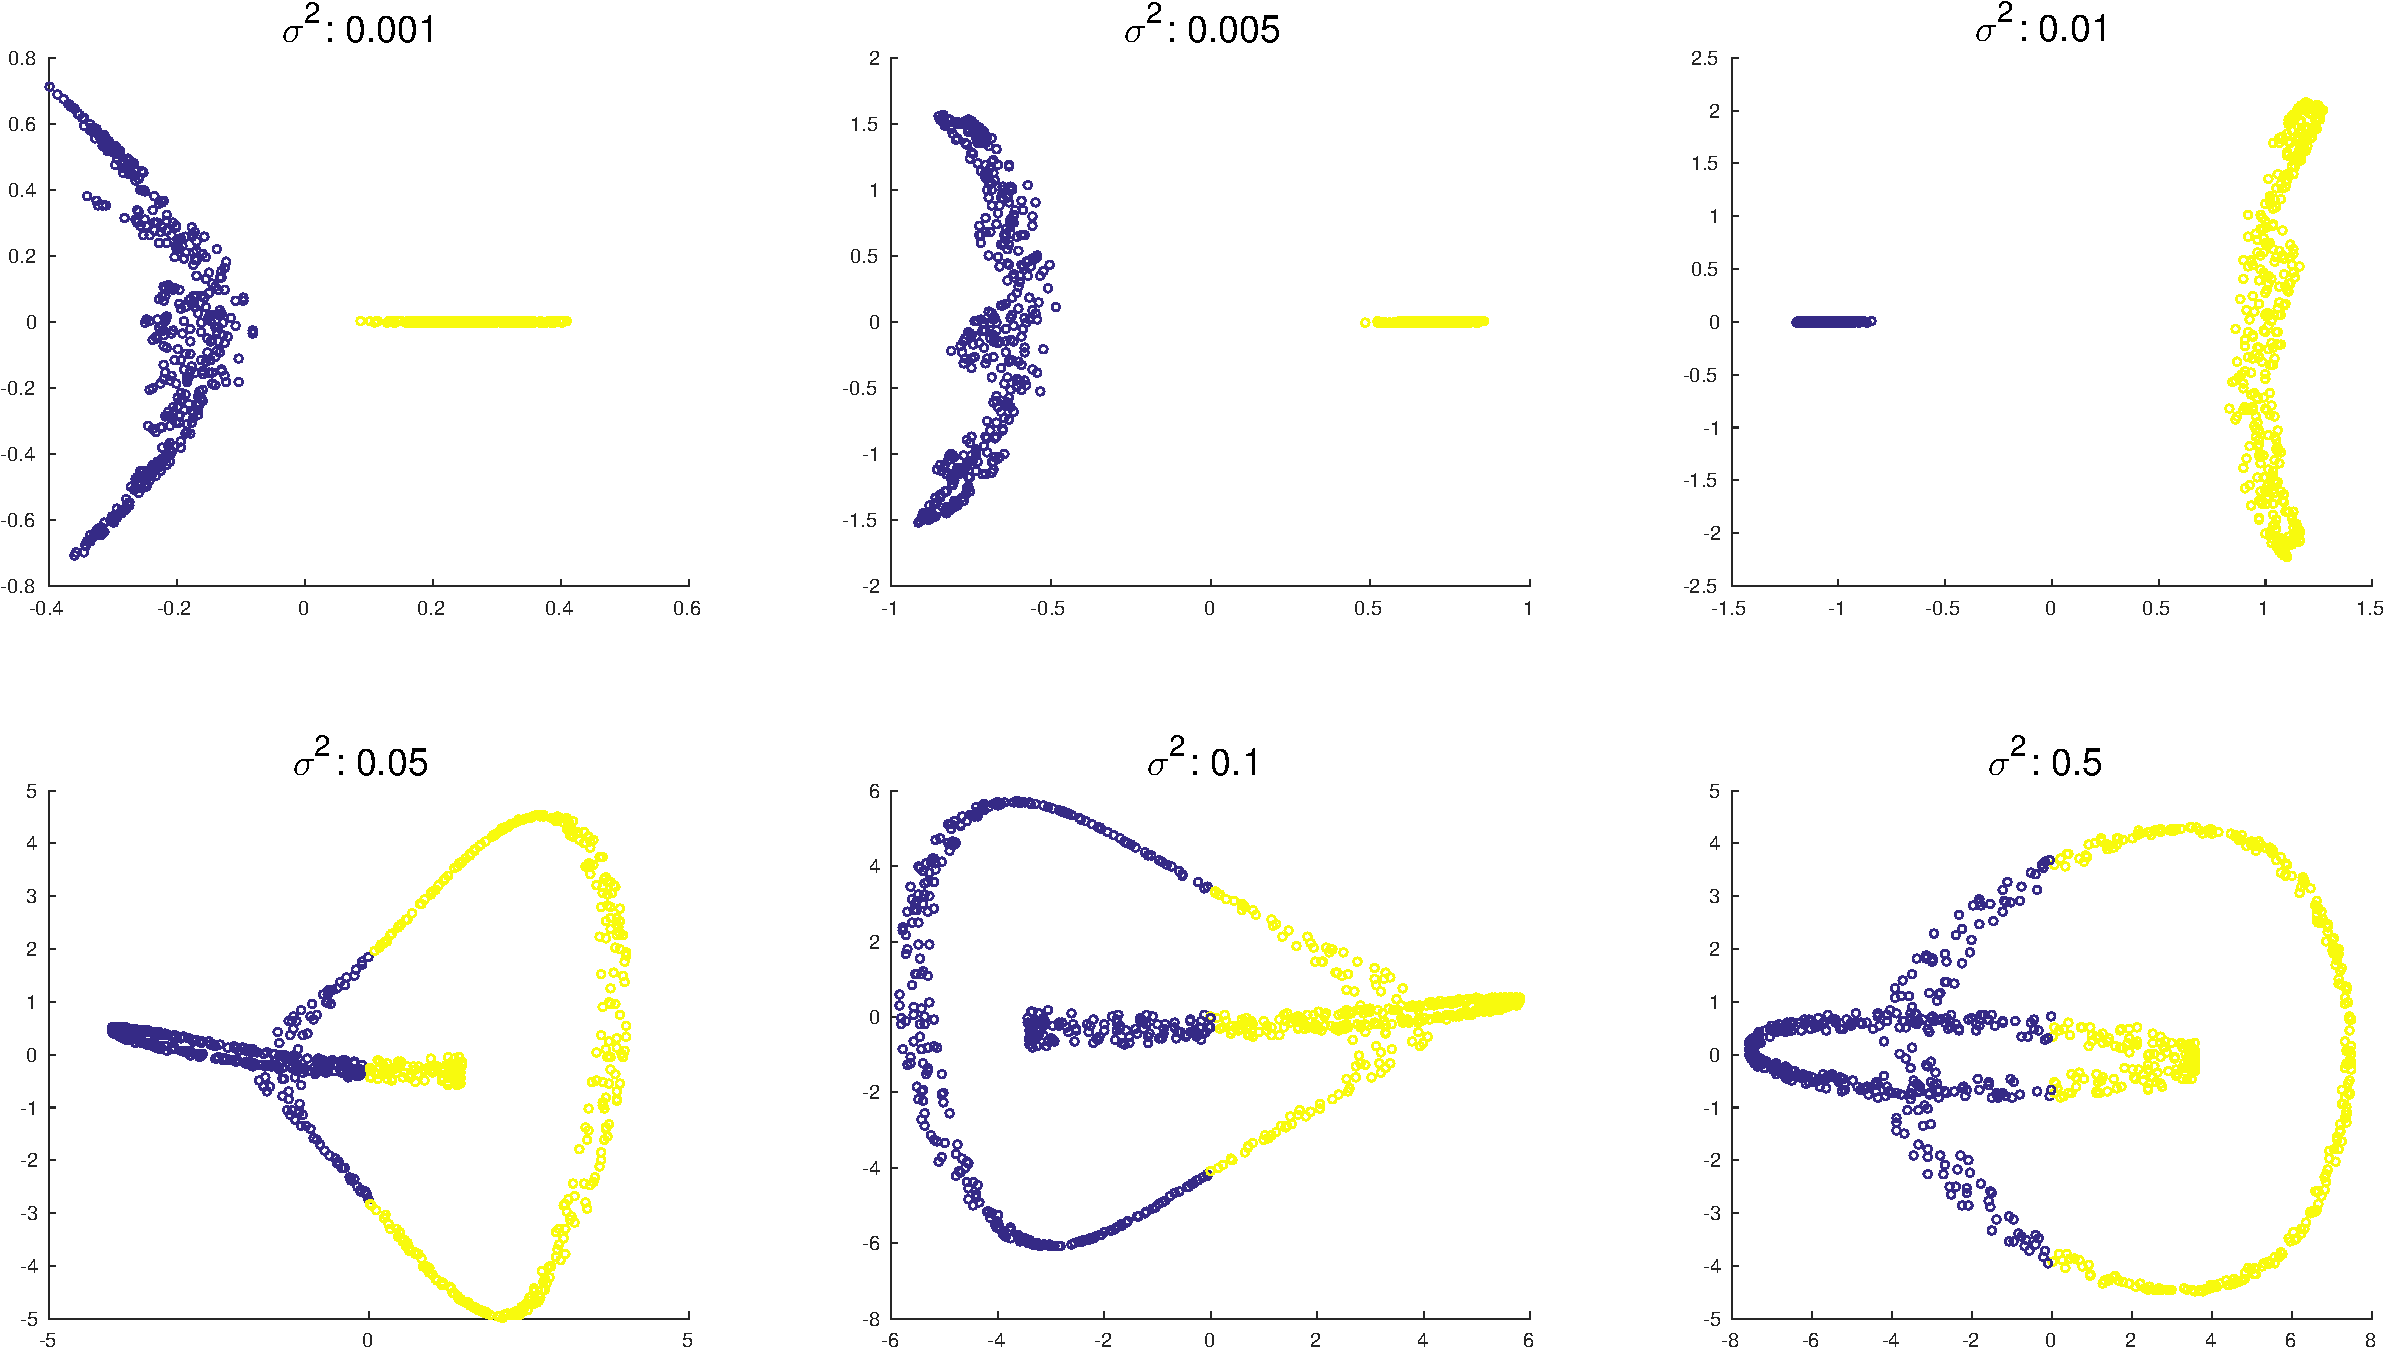
\includegraphics[scale=.40]{sclustering_origcl2.pdf}
  \caption{Clustering 2}
  \label{fig:sclustering_origcl2}
\end{figure}

\section{Fixed-size LS-SVM}

\section{Applications}

\subsection{Handwritten Digit Denoising}

\subsection{Shuttle (statlog)}

\subsection{California}

%\bibliographystyle{ieeetr} \bibliography{bib-db}
\end{document}
